\documentclass[a4paper, oneside]{discothesis}

\usepackage[utf8]{inputenc}
\usepackage[T1]{fontenc}
\usepackage{CJKutf8}
\usepackage{tikz}
\usetikzlibrary{shapes,arrows,positioning}


%%%%%%%%%%%%%%%%%%%%%%%%%%%%%%%%%%%%%%%%%%%%%%%%%%%%%%%%%%%%%%%%%%%%%%%%%%%%%%%%%%%%%%%%%%%%%%%%%
% DOCUMENT METADATA

\thesistype{Towards more data-driven, and less biased decisions in startup investing with AI workflows} % Master's Thesis, Bachelor's Thesis, Semester Thesis, Group Project
\title{Moon AI: automating VC}

\author{Angelo Giacco}
\email{agiacco@ethz.ch}

\institute{ETH AI Centre \\[2pt]
ETH Zürich}

\logo{\includegraphics[width=0.2\columnwidth]{figures/eth_ai_center}}

\supervisors{Isabelle Siegrist\\[2pt] Prof. Dr. Elliott Ash}

% Optionally, keywords and categories of the work can be shown (on the Abstract page)
%\keywords{Keywords go here.}
%\categories{ACM categories go here.}

\date{\today}

%%%%%%%%%%%%%%%%%%%%%%%%%%%%%%%%%%%%%%%%%%%%%%%%%%%%%%%%%%%%%%%%%%%%%%%%%%%%%%%%%%%%%%%%%%%%%%%%%

\begin{document}

\frontmatter % do not remove this line
\maketitle

\cleardoublepage

\begin{acknowledgements}
	I would like to express my sincere gratitude to several individuals who have been instrumental in the completion of this thesis. First and foremost, I extend my heartfelt thanks to my advisor, Isabelle Siegrist, for her invaluable guidance, and to Professor Elliott Ash for his mentorship. It was only by pure chance that we collaborated, but I am very grateful that we did.

A big thanks to everyone at Beugi that made my year in Switzerland so wonderful and full of hike/ski days.

I owe as always a special debt of gratitude to my family for their love and support.

    \begin{CJK*}{UTF8}{gbsn}
最后,我要特别感谢我的伴侣萧庭恩。她始终如一的支持和对我的信任是我前进的动力。\clearpage\end{CJK*}
\end{acknowledgements}



\begin{abstract}
    The venture capital (VC) industry has in recent years experienced a significant shift towards a solo General Partner (GP) model, where a single partner, often a successful former founder or early hire at a unicorn, raises a fund to invest in upcoming entrepreneurs. Solo-GPs are more agile but lack the platform services and in depth analysis available to VC firms with large teams. Simultaneously, Large Langauge Models (LLMs) have emerged as powerful multi-task learners. This has led to the emergence of AI-copilots powered by LLMs for multi-task reasoning emerging in various verticals. 
    
    This thesis explores the creation of a new product: MoonAI. MoonAI is a venture investing copilot designed to empower solo GPs and traditional VC firms alike, by providing a copilot capable of emulating a team of analysts. By employing large language models for reasoning, structured output to guide agents, and matryoshka embeddings to semantically search the internet, the system extracts relevant signals for startup investing from vast amounts of unstructured data publicly available on the internet. The end result is a tool that helps assist in sourcing startups and generating investment memos.
    
    MoonAI can be customized to align with various investment hypotheses, supporting solo GPs in their sourcing and due diligence processes and removing the need for duplicate platform teams at each VC firm. MoonAI aims to evolve into a comprehensive data science and investing platform.
    
    By creating this adaptable infrastructure, MoonAI seeks to democratise access to high-quality investment platforms, encourage data-driven investing, and thereby democratise access to capital. The project's core thesis posits that successful VC firms and especially solo-GPs will increasingly rely on automated research analysts to support upcoming entrepreneurs, with MoonAI positioning itself at the forefront of this transformation.
    
    This thesis provides an overview of the advances in Natural Language Processing that make MoonAI possible, an overview of the VC industry, and details how the product was built. 
\end{abstract}


\begin{zusammenfassung}
Die Venture-Capital-Branche (VC) hat in den letzten Jahren eine bedeutende Verlagerung hin zu einem Modell mit einem einzelnen General Partner (GP) erlebt, bei dem erfolgreiche ehemalige Gründer aufstrebende Unternehmer unterstützen.
Gleichzeitig haben sich Large Language Models (LLMs) als leistungsfähige Multi-Task-Lerner etabliert. Dies hat dazu geführt, dass in verschiedenen Bereichen KI-Copiloten entstanden sind, die sich auf LLMs für Multi-Task-Reasoning stützen.
CopyDiese Arbeit untersucht die Entwicklung eines neuen Produkts, MoonAI, eines innovativen Venture-Investing-Copiloten, der sowohl einzelne GPs als auch traditionelle VC-Firmen unterstützen soll, indem er als Copilot fungiert, der ein Team von Analysten emulieren kann.
Durch den Einsatz von Large Language Models für Reasoning, strukturierte Ausgaben zur Steuerung von Agenten und Matryoshka-Embedding für semantische Internetsuchen extrahiert das System relevante Signale für Startup-Investitionen aus großen Mengen unstrukturierter Internetdaten.

Derzeit als Memo-Generierungstool mit einem einfachen CRM-Layout verpackt, strebt MoonAI an, sich zu einer umfassenden Plattform für Data Science und Investitionen zu entwickeln. Das System kann an verschiedene Investitionshypothesen angepasst werden, um einzelne GPs bei ihren Sourcing- und Due-Diligence-Prozessen zu unterstützen und die Notwendigkeit von doppelten Plattform-Teams in jeder VC-Firma zu eliminieren.

Durch die Schaffung dieser anpassungsfähigen Infrastruktur zielt MoonAI darauf ab, den Zugang zu hochwertigen Investitionsplattformen zu demokratisieren, datengetriebenes Investieren zu fördern und dadurch den Zugang zu Kapital zu demokratisieren. Die Kernthese des Projekts postuliert, dass erfolgreiche VC-Firmen und insbesondere einzelne GPs zunehmend auf automatisierte Research-Analysten zurückgreifen werden, um aufstrebende Unternehmer zu unterstützen, wobei sich MoonAI an der Spitze dieser Transformation positioniert.

Diese Arbeit bietet einen Überblick über die Fortschritte in der Natürlichen Sprachverarbeitung, die MoonAI ermöglichen, einen Überblick über die VC-Branche und detaillierte Informationen darüber, wie das Produkt entwickelt wurde.
\end{zusammenfassung}

\tableofcontents

\mainmatter % do not remove this line

% Start writing here
\chapter{Introduction}

The venture capital (VC) industry stands at the forefront of innovation, playing a crucial role
in identifying and nurturing startups that have the potential to disrupt industries and drive
economic growth. Indeed, Acs et al. ~\cite{acs} find that startups are key catalysts for economic growth, 
not only creating new markets but also stimulate competition and innovation in existing ones, bringing economic dynamism across multiple sectors. 

The VC industry invests in startups with significant potential to disrupt industries and drive economic growth. 
VC investments returns follow a power law distribution, with a long tail of successful investments. 
Indeed, a study of 21,000 financings from 2004-2013 by Correlation Ventures found that 65\% of financings fail to return 1x capital ~\cite{levine2014venture}, 
thus the remaining 35\% must return significantly more to generate a net-return that is acceptable. 
VCs rely on a small number of portfolio investments to achieve outstanding paybacks: enough to cover for losses and
still produce substantial profits. To generate these substantial outcomes, startups rely on the external funding from VCs
to achieve rapid growth, often depicted by a "hockey stick" growth curve ~\cite{marmer}.

The power law nature of startups means that the competition to get on the best deals is incredibly intense, and those 
deals are also the only ones that matter. The top 2\% of VC funds capture 95\% of industry
returns ~\cite{bai}. Particularly at the earliest stage of the investment lifecycle (pre- Series A), there is a scarcity of
reliable information ~\cite{dellermann}. As a result, VCs often rely heavily on human judgment which is prone to bias. 
This may yield sub-optimal decisions ~\cite{cummingdai} and could explain why women-led startups only received 2.1\% of all venture capital invested in 2023 ~\cite{pitchbook2024vc}.
Traditionally, VC firms have relied heavily on human intuition, personal networks, and experience
to identify promising investment opportunities. While this approach has yielded success, it is
not without limitations. Human decision-making is susceptible to biases, inconsistencies, and the
constraints of processing vast amounts of information.

VCs have increasingly adopted data-driven investing practices to combat these biases. 
Traditional gradient boosting approaches have been used successfully, and in recent years the growth of data volume has ushered deep learning (DL) into the industy ~\cite{eqt}.
For example, graph neural networks have been used to predict a startup's success based on its links to a wider startup ecosystem ~\cite{korea}. 
These models can integrate diverse data sources, including structured information about startups, founders, and investors ~\cite{corea}, as well as unstructured data from social networks and web sources. 
Preliminary findings suggest that data-driven VCs may be more likely to back founders from underrepresented backgrounds, potentially addressing systemic biases in the industry ~\cite{futureVC}.

In recent years, the venture capital landscape has witnessed a significant shift with the emergence of solo general partners (GPs) and difficult fundraising conditions for non-elite VC firms. 
Unlike traditional VC firms that often require consensus among multiple partners, solo GPs can make investment decisions quickly and independently, which is particularly valuable in competitive deal environments where rapid decision-making can be crucial.
In contrast, the formation of new traditional VC firms has slowed in recent years. This can be attributed to several factors, including the trend towards larger fund sizes, which makes it challenging for new firms to compete and gain traction with the returns from the VC industry becoming concentrated among well-established firms that enjoy significant advantages in deal flow and fundraising. 
The difficulty of smaller VCs to raise funds means they will have less resources for research, contributing to their worse performance.

In addition, solo GPs have extremely limited resources which may amplify the issues of bias and incomplete information in the investment process, forcing them to  focus on a narrower pool of potential investments, potentially overlooking promising opportunities outside their immediate network (Huang et al., 2020). 
Furthermore, without the resources to explore a wide range of sectors or geographies, solo GPs might gravitate towards familiar industries or founder profiles, potentially limiting the diversity of their investment portfolios (Gompers et al., 2021) and limiting opportunities for under represented founders.
In addition, the agility of solo GPs will intensify the competition and rush to produce term sheets for 'hot' startups. 

In response to these challenges, a project at the ETH AI Center of ETH Zurich aims to introduce automation to VC firms and facilitate the adoption of data-driven investing practices. 
The project focuses on developing an AI-powered tool for generating investment memoranda. This approach aims to streamline the decision-making process for investment analysts, significantly reducing the time spent on screening potential investments. 
Utilizing multimodal data and state-of-the-art language models, the system aggregates diverse data sources, including pitch decks, financial data, and web information, to provide a comprehensive analysis of investment opportunities.
Furthermore, this project introduces tools for data-driven investing that aim to reduce bias in the investment process by incorporating objective insights, broadening investment scope, identifying overlooked startups, informing decisions with diverse data points, and standardizing evaluation processes. Developing the MoonAI product is the first phase of this project; subsequent research will analyse its ability to reduced bias decision making. 

The potential impact of such a tool is multifaceted. First, it addresses the resource disparity
between solo GPs/smaller VC firms and larger VC firms, potentially democratizing access to high-quality investment
analysis. Second, it introduces a data-driven approach to complement human intuition in the
investment process, potentially reducing biases and improving decision-making accuracy
~\cite{dellermann}. Finally, by streamlining the sourcing and evaluation processes, MoonAI
could allow VCs to consider a broader range of startups by reducing the cognitive load of analysing a startup, potentially leading to a more diverse
and inclusive investment landscape (Brush et al., 2019).

While the VC industry has been facing challenges, Large Language Models (LLMs) have emerged as powerful tools capable of multi-task reasoning and processing vast amounts of
unstructured data (Brown et al., 2020) and transformed the field of Natural Language Processing (NLP). These advancements have led to the development of
AI-powered copilots in various industries, augmenting human capabilities and decision-making processes.
 Large Language Models (LLMs) are particularly well-suited to be a venture capital copilot and decision-making support for several key reasons. 
Firstly, LLMs excel at pattern matching, a crucial skill in the venture capital industry. They can analyze vast amounts of unstructured data from various sources, identifying trends, similarities, and potential success indicators that might not be immediately apparent to human analysts.
They can rapidly process and synthesize information from a wide range of publicly available sources, including news articles, social media, academic publications, and industry reports. This ability enables a comprehensive understanding of a startup's market position, competitive landscape, and potential growth trajectory without relying solely on information provided by the startup itself.
Furthermore, LLMs offer simple yet powerful workflow automation capabilities. They can streamline many time-consuming aspects of the venture capital process, such as initial startup screening, report generation, and even preliminary financial analysis. By automating these routine tasks, LLMs free up valuable time for venture capitalists to focus on higher-level strategic decisions and relationship building with promising founders. This efficiency gain is particularly beneficial for solo GPs or smaller VC firms with limited resources, allowing them to compete more effectively with larger, more established firms.
The combination of these capabilities makes LLMs an ideal tool for augmenting human decision-making in venture capital. They can provide data-driven insights, reduce information asymmetry, and increase the overall efficiency of the investment process. As the venture capital landscape continues to evolve and become more competitive, the integration of LLMs into investment workflows has the potential to significantly enhance the accuracy, speed, and scope of investment decisions, ultimately leading to better outcomes for both investors and entrepreneurs.

The emergence of Large Language Models (LLMs) represents a significant milestone in the fields of artificial intelligence and natural language processing. The development of these models can be traced through several key stages, each marking a crucial advancement in the technology.
The foundations of natural language processing can be traced back to the 1950s, with Alan Turing's seminal work on the "Turing Test" ~\cite{turing1950computing}. Over the subsequent decades, rule-based systems and statistical methods formed the basis of early NLP research, laying the groundwork for future advancements.
The early 2010s saw a resurgence of interest in neural networks, thanks to the ability to train on GPUs, leading to breakthroughs such as word2vec ~\cite{mikolov2013efficient}. This innovation allowed words to be represented as dense vectors, capturing semantic relationships in a way that significantly enhanced the capabilities of NLP systems.
Between 2014 and 2017, the introduction of sequence-to-sequence models ~\cite{sutskever2014sequence} and the attention mechanism ~\cite{bahdanau2014neural} marked another leap forward. These advancements significantly improved machine translation and other NLP tasks.
A pivotal moment came in 2017 with the publication of "Attention is All You Need" ~\cite{vaswani2017attention}, which introduced the Transformer architecture. This innovation became the foundation for modern LLMs, as the transformer architecture allowed for highly parallel 
The years 2018 and 2019 saw the emergence of the pre-training and fine-tuning paradigm. Models such as BERT ~\cite{devlin2018bert} and GPT ~\cite{radford2018improving} demonstrated the power of pre-training on large corpora followed by task-specific fine-tuning, setting new benchmarks in NLP performance.
From 2020 onwards, the focus shifted to scaling up these models. GPT-3 ~\cite{brown2020language} demonstrated that increasing model size and training data could lead to emergent abilities, a trend that has continued with subsequent models such as PaLM, Chinchilla, and GPT-4.
Most recently, from 2022 onwards, there has been a growing emphasis on instruction tuning and alignment. Models like InstructGPT and ChatGPT have highlighted the importance of aligning LLMs with human intent, often through techniques such as reinforcement learning from human feedback (RLHF) ~\cite{ouyang2022training}.
The latest developments in the field include the exploration of agent simulacra and agentic workflows, pushing the boundaries of what LLMs can achieve in terms of task completion and decision-making processes.


This thesis explores the intersection of these trends through the development of MoonAI, an
AI-powered venture investing copilot designed to empower both solo GPs and traditional VC firms.
By leveraging state-of-the-art LLMs, structured output for guided reasoning, advanced
semantic search capabilities, and agentic workflows, MoonAI aims to speed up the startup evaluation process and remove repetitive tasks from a VC. The
system is designed to extract relevant signals for startup investing from the vast pool of
publicly available unstructured data on the internet, assisting in sourcing startups and
generating comprehensive investment memos. By addressing these questions and developing a practical tool for the VC industry, this thesis
aims to contribute to the ongoing dialogue about the role of AI in financial decision-making and
its potential to reshape the startup ecosystem. The following chapters will delve into the
technical foundations of Large Language Models, a review of the Venture Capital industry, and evaluate the MoonAI platform. 

\chapter{Natural Language Processing}

In this section, the recent in advances in Natural Language Processing will be discussed. First, we will consider the basics of machine learning, 
consider the standard, non-deep learning approaches to NLP used in the past and discuss the advances that have been made in recent years.

Many of these advances have been possible due to the parallelizability of training thanks to the Transformer architecture which make use of advances in GPUs. 
How GPUs are able to parallelize the training of large language models is beyond the scope of this overview, but it is important to note that this is a significant
advance that has revolutionized the field of NLP. It can be summarised as follows: GPUs have significantly accelerated the training of transformer-based models by leveraging their ability to perform massive parallel computations, which make them ideal for matrix multiplications, the operation underpinning the self-attention mechanism in transformers and the feed-forward layers. 
GPUs excel at these tasks due to their architecture, which is designed to handle many simple calculations simultaneously.
This GPU-driven acceleration has been a key factor in enabling the training of increasingly large and complex language models, pushing the boundaries of what's possible in NLP.

Before we consider the essentials of machine learning that enable the training of large language models, let us first specify the objective of a large language model more clearly. 
This will also motivate the use of the Transformer architecture, and clarify why other methods, from n-gram based approaches to other flavours of DL like recurrent neural networks, are not suited for the task.

\begin{theorem}[Language Modelling Objective] \label{thm:first theorem}
    Given an alphabet $\Sigma$ and a distinguished end-of-sequence symbol $\texttt{eos} \notin \Sigma$, a
    language model is a collection of conditional probability distributions $p(y \mid w)$ for $y \in \Sigma \cup \{\texttt{eos}\}$ and $\w \in \Sigma^*$,
    the Kleene closure of $\Sigma$.
\end{theorem}

We therefore can obtain the probability of a string according to a particular language model by autoregressively factorising:

\begin{equation}
    P(w) = P(w_1, \ldots, w_n) =  P(\texttt{EOS} \mid w) \cdot \prod_{i=1}^n P(w_i \mid w_1, \ldots, w_{i-1}) 
\end{equation}

With the objective of crafting a model able to learn this function p in mind, let us begin our exploration of machine learning. 

\section{Modelling Data}

This thesis assumes some familiarity with the basics of machine learning. Nevertheless, a brief summary is provided here to establish a foundation for the subsequent discussions.

In classical computer programming, humans define a set of explicit rules and provide input data. The computer then processes this data according to the predefined rules to produce an output. 
This approach works well for problems with clear, unchanging rules and predictable inputs.
Machine learning, on the other hand, inverts this paradigm. Instead of explicitly programming rules, humans provide a large dataset of input-output pairs (often referred to as training data). 
The machine learning algorithm then attempts to learn the underlying patterns or rules that map the inputs to the outputs. 
This learned model can then be used to make predictions or decisions on new, unseen data.
The key advantage of machine learning is its ability to handle complex, non-linear relationships in data and to adapt to new patterns without being explicitly reprogrammed. 
This makes it particularly useful for tasks like natural language processing, where the rules governing language use are clearly too complex and nuanced to be explicitly coded.

\subsection{Losses}
To begin our search for a model that best describes the underlying patterns in our data, it is necessary to find a way of describing how accurate our model's predictions are.
This is done by defining a loss function that measures the difference between the model's predictions and the ground-truth values.

In the context of natural langauge processing where have the option of predicting multiple labels for a single input, an evident choice for the loss function is cross-entropy which 
has its basis in information theory as a measure of the difference between two probability distributions.

The cross-entropy loss, denoted as $H(p,q)$, for a classification task with $C$ classes is defined as:

\begin{equation}
    H(p,q) = -\sum_{i=1}^C p(i) \log q(i)
\end{equation}

where $p(i)$ is the true probability distribution (usually a one-hot encoded vector for the true class) and $q(i)$ is the predicted probability distribution from the model.

For binary classification, this simplifies to:

\begin{equation}
    H(p,q) = -[y \log(\hat{y}) + (1-y) \log(1-\hat{y})]
\end{equation}

where $y$ is the true label (0 or 1) and $\hat{y}$ is the predicted probability of the positive class.

In the context of language modeling, where we're predicting the next token in a sequence, the cross-entropy loss is calculated over the entire vocabulary at each step:

\begin{equation}
    L = -\sum_{t=1}^T \sum_{v=1}^V y_{t,v} \log(\hat{y}_{t,v})
\end{equation}

where $T$ is the sequence length, $V$ is the vocabulary size, $y_{t,v}$ is 1 if token $v$ is the true next token at position $t$ and 0 otherwise, and $\hat{y}_{t,v}$ is the model's predicted probability for token $v$ at position $t$.

Minimizing this loss encourages the model to assign higher probabilities to the correct next tokens in the training data, thus learning the underlying patterns of the language.

Given a neural network architecture $\mathcal{A}$, it induces a parameter space $\Theta \subset \mathbb{R}^d$, where $d$ is the total number of parameters in the network. Each point $\theta \in \Theta$ represents a specific configuration of the network's parameters.

Let $\mathcal{L}: \Theta \rightarrow \mathbb{R}$ be the loss function that measures the performance of the model on the given task. The goal of training the neural network can then be formally expressed as an optimization problem:

\begin{equation}
    \theta^* = \arg\min_{\theta \in \Theta} \mathcal{L}(\theta)
\end{equation}

where $\theta^*$ represents the optimal set of parameters that minimizes the loss function over the entire parameter space $\Theta$. This optimization problem encapsulates the essence of training a neural network: finding the configuration of parameters that yields the best performance according to the chosen loss function.


\subsection{Optimising Parameters}

\subsubsection{Gradient Descent}

Gradient descent is a fundamental optimization algorithm used in training neural networks. It iteratively adjusts the model parameters in the direction of steepest descent of the loss function. The basic update rule for gradient descent is:

\begin{equation}
    \theta_{t+1} = \theta_t - \eta \nabla \mathcal{L}(\theta_t)
\end{equation}

where $\theta_t$ are the parameters at iteration $t$, $\eta$ is the learning rate, and $\nabla \mathcal{L}(\theta_t)$ is the gradient of the loss function with respect to the parameters.

Stochastic Gradient Descent (SGD) is a variant that computes the gradient using only a small subset (mini-batch) of the training data in each iteration, making it more computationally efficient for large datasets.

\subsubsection{Automatic Differentiation}

Automatic Differentiation (AutoDiff) allows for efficient and accurate computation of gradients, which are essential for optimization algorithms like gradient descent.

Mathematically, for a composite function $f(g(x))$, the chain rule states:

\begin{equation}
    \frac{df}{dx} = \frac{df}{dg} \cdot \frac{dg}{dx}
\end{equation}

AutoDiff systems leverage this principle to compute gradients through arbitrarily complex computational graphs. Modern deep learning frameworks like PyTorch and TensorFlow have built-in AutoDiff capabilities, which greatly simplify the implementation of new models and training procedures. These systems maintain a computational graph of operations and use it to automatically compute gradients, enabling efficient training of large-scale neural networks, allows researchers to focus on designing network architectures and loss functions, while the AutoDiff system handles the intricate details of gradient computation.

Several advanced optimization algorithms have been developed to improve upon basic SGD. Momentum adds a fraction of the previous update to the current one, helping to accelerate convergence and reduce oscillations:
\begin{equation}
    v_{t+1} = \gamma v_t + \eta \nabla \mathcal{L}(\theta_t)
\end{equation}
\begin{equation}
    \theta_{t+1} = \theta_t - v_{t+1}
\end{equation}
where $\gamma$ is the momentum coefficient.RMSprop adapts the learning rate for each parameter based on the historical gradient magnitudes:
\begin{equation}
    s_{t+1} = \beta s_t + (1-\beta)(\nabla \mathcal{L}(\theta_t))^2
\end{equation}
\begin{equation}
    \theta_{t+1} = \theta_t - \frac{\eta}{\sqrt{s_{t+1} + \epsilon}} \nabla \mathcal{L}(\theta_t)
\end{equation}
where $\beta$ is the decay rate and $\epsilon$ is a small constant for numerical stability.
The most widely adopted optimizer in practice, Adam, combines ideas from momentum and RMSprop, maintaining both a running average of gradients and their squared values:
\begin{equation}
    m_{t+1} = \beta_1 m_t + (1-\beta_1)\nabla \mathcal{L}(\theta_t)
\end{equation}
\begin{equation}
    v_{t+1} = \beta_2 v_t + (1-\beta_2)(\nabla \mathcal{L}(\theta_t))^2
\end{equation}
\begin{equation}
    \theta_{t+1} = \theta_t - \frac{\eta}{\sqrt{\hat{v}_{t+1}} + \epsilon} \hat{m}_{t+1}
\end{equation}
where $\hat{m}_{t+1}$ and $\hat{v}_{t+1}$ are bias-corrected estimates of $m_{t+1}$ and $v_{t+1}$ respectively.

These advanced optimizers often lead to faster convergence and better generalization in practice.

\subsubsection{Initialisation}

Proper initialization of neural network parameters is crucial for effective training. Two popular initialization methods have been developed to address this need: Xavier Initialization and He Initialization.

Xavier Initialization, proposed by Glorot and Bengio, is designed to maintain the variance of activations and gradients across layers. For a layer with $n_{in}$ input units and $n_{out}$ output units, weights are initialized from a uniform distribution:

\begin{equation}
    W \sim U\left(-\sqrt{\frac{6}{n_{in} + n_{out}}}, \sqrt{\frac{6}{n_{in} + n_{out}}}\right)
\end{equation}

This initialization works well for layers with linear activations or tanh activations, helping to prevent the vanishing or exploding gradient problem in deep networks.

He Initialization, proposed by He et al., is particularly suited for layers with ReLU activations. In this method, weights are initialized from a normal distribution:

\begin{equation}
    W \sim N\left(0, \sqrt{\frac{2}{n_{in}}}\right)
\end{equation}

This approach helps maintain the variance of the outputs, which is especially important for deep networks with ReLU activations, as it prevents vanishing or exploding gradients.

Both Xavier and He initialization methods aim to set initial parameters that neither shrink nor amplify the input signal excessively. By doing so, they facilitate smoother optimization and faster convergence during the training process, ultimately leading to more effective and efficient neural network models \cite{glorot2010understanding, he2015delving}.

\subsubsection{Normalisation}

In addition to these initialization techniques, normalization methods such as Batch Normalization and Layer Normalization are also employed to address similar issues during training.

Batch Normalization, introduced by Ioffe and Szegedy \cite{ioffe2015batch}, normalizes the inputs of each layer for each mini-batch:
\begin{equation}
    \hat{x} = \frac{x - \mu_B}{\sqrt{\sigma_B^2 + \epsilon}}
\end{equation}
where $\mu_B$ and $\sigma_B^2$ are the mean and variance of the mini-batch, and $\epsilon$ is a small constant for numerical stability. Batch Normalization helps reduce internal covariate shift, allows higher learning rates, and acts as a regularizer.

Layer Normalization, proposed by Ba et al. \cite{ba2016layer}, normalizes the inputs across the features:
\begin{equation}
    \hat{x} = \frac{x - \mu}{\sqrt{\sigma^2 + \epsilon}}
\end{equation}
where $\mu$ and $\sigma^2$ are the mean and variance computed over all features for each data point. Layer Normalization is particularly useful for recurrent neural networks and does not depend on batch size.

Both Batch Normalization and Layer Normalization help stabilize the distribution of layer inputs throughout training, mitigating the vanishing/exploding gradient problem and enabling more efficient training of deep neural networks \cite{santurkar2018does}. These techniques complement initialization methods by maintaining appropriate scaling of activations and gradients throughout the network during the entire training process.

\subsection{Regularisation}

Regularisation techniques are employed to prevent overfitting and improve the generalization of neural networks \cite{goodfellow2016deep}. Overfitting occurs when a model learns the training data too well, including its noise and peculiarities, leading to poor performance on unseen data. This happens because the model becomes too complex and starts to memorize the training examples rather than learning general patterns. Regularisation methods aim to strike a balance between fitting the training data and maintaining simplicity to ensure good performance on new, unseen data \cite{bishop2006pattern}. Some common regularisation methods include:

Dropout randomly "drops out" a proportion of neurons during training, forcing the network to learn more robust features \cite{srivastava2014dropout}. During inference, all neurons are used but their outputs are scaled:

\begin{equation}
    y = f(Wx) \odot m, \quad m_i \sim \text{Bernoulli}(p)
\end{equation}

where $p$ is the probability of keeping a neuron active.

Early Stopping monitors the validation error during training and stops when it starts to increase, preventing the model from overfitting to the training data \cite{prechelt1998early}.

Weight Decay adds a penalty term to the loss function based on the L2 norm of the weights \cite{krogh1992simple}:

\begin{equation}
    \mathcal{L}_{new}(\theta) = \mathcal{L}(\theta) + \lambda \|\theta\|_2^2
\end{equation}

where $\lambda$ is the weight decay coefficient. This encourages smaller weights and simpler models.

Data Augmentation artificially increases the size of the training set by applying transformations to existing data points, helping the model learn invariances and improving generalization \cite{shorten2019survey}.

These regularisation techniques, often used in combination, help in training more robust models that perform well on unseen data \cite{kukavcka2017regularization}.

\section{Historical Language Representations}

Natural Language Processing (NLP) has evolved significantly over the years, with various techniques developed to represent and analyze textual data. This section explores the historical approaches to language representation that laid the foundation for modern NLP methods. We will discuss three key techniques that were widely used before the advent of deep learning and neural network-based models: N-grams, Word Document Frequency, and Topic Modelling. These methods played crucial roles in tasks such as text classification, information retrieval, and document analysis, and their principles continue to influence contemporary NLP approaches.

\subsection{N-grams}
N-grams are contiguous sequences of n items from a given sample of text or speech. In the context of natural language processing, these items are typically words or characters. N-grams have been a fundamental technique in language modeling and various NLP tasks for several decades.

The concept of n-grams was introduced in the early days of computational linguistics. One of the seminal papers that popularized the use of n-grams in language modeling is "A Mathematical Theory of Communication" by Claude Shannon (1948), which laid the foundation for information theory and introduced the idea of using probabilistic models for language.

N-grams achieved state-of-the-art performance in many NLP tasks throughout the 1990s and 2000s. For instance, the paper "An Empirical Study of Smoothing Techniques for Language Modeling" by Chen and Goodman (1996) demonstrated the effectiveness of various n-gram models for language modeling tasks. Another influential work, "A Bit of Progress in Language Modeling" by Goodman (2001), showed how n-gram models could be extended and improved for better performance.

Google Translate, one of the most widely used machine translation systems, initially relied heavily on n-gram models. Specifically, it used a 5-gram language model, as described in the paper "Large Language Models in Machine Translation" by Brants et al. (2007). This approach allowed Google Translate to capture local context and produce more fluent translations compared to earlier rule-based systems.

However, despite their historical success, n-grams have limitations that make them less suitable for modern language models. One significant limitation is their restricted context, as n-grams can only capture local context within a fixed window size. This constraint makes it challenging to model long-range dependencies in language, which are crucial for understanding complex sentences and maintaining coherence across paragraphs. Another issue is sparsity; as n increases, the number of possible n-grams grows exponentially, leading to data sparsity issues. This makes it difficult to estimate probabilities for rare or unseen n-grams accurately. N-gram models also lack semantic understanding, treating words as discrete symbols without considering their meaning or relationships. This limitation hinders their ability to capture semantic similarities between words or phrases. Additionally, traditional n-gram models operate on a fixed vocabulary, making it difficult to handle out-of-vocabulary words or adapt to new domains. Lastly, the memory requirements for n-gram models can be substantial, as storing probabilities for all possible n-grams can be memory-intensive, especially for large values of n.

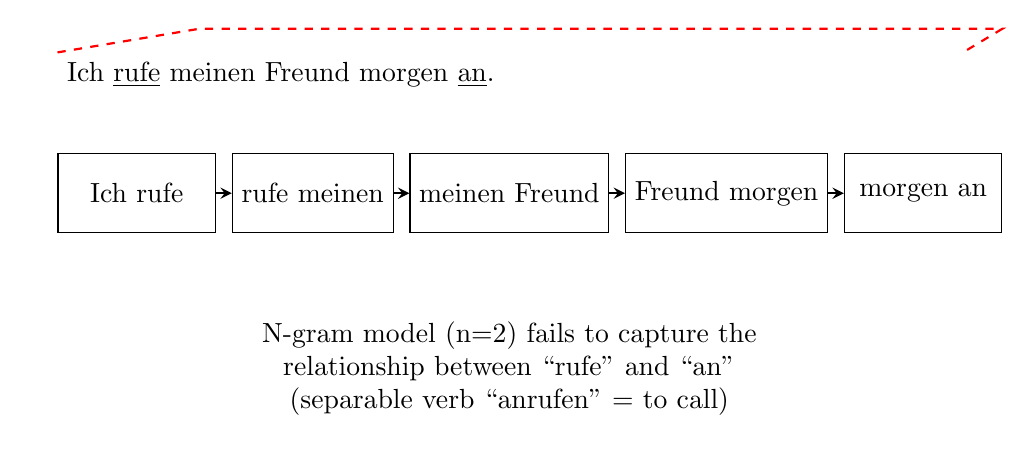
\begin{tikzpicture}[
    box/.style={draw, rectangle, minimum width=2cm, minimum height=1cm},
    arrow/.style={->, >=stealth, thick},
    node distance=0.5cm
]

% The sentence
\node[anchor=west] (sentence) at (0,0) {Ich \underline{rufe} meinen Freund morgen \underline{an}.};

% N-gram boxes
\node[box, below=1cm of sentence.west, anchor=north west] (box1) {Ich rufe};
\node[box, right=0.2cm of box1] (box2) {rufe meinen};
\node[box, right=0.2cm of box2] (box3) {meinen Freund};
\node[box, right=0.2cm of box3] (box4) {Freund morgen};
\node[box, right=0.2cm of box4] (box5) {morgen an};

% Arrows
\foreach \i in {1,...,4}
    \draw[arrow] (box\i) -- (box\the\numexpr\i+1);

% Explanation
\node[text width=12cm, below=1cm of box3, align=center] (explanation) {
    N-gram model (n=2) fails to capture the relationship between ``rufe'' and ``an''\\
    (separable verb ``anrufen'' = to call)
};

% Highlighting the issue
\draw[red, thick, dashed] (sentence.north west) -- ++(1.8cm,0.3cm) -- ++(10.2cm,0) -- ++(-0.5cm,-0.3cm);

\end{tikzpicture}

These limitations have led to the development of more advanced techniques, such as neural network-based language models and transformer architectures, which can capture longer-range dependencies, understand semantic relationships, and generate more coherent and contextually appropriate text.

\subsection{Document Term Matrices}
Document Term Matrices (DTMs) are a fundamental representation in natural language processing and information retrieval. They provide a structured way to represent a collection of documents as a matrix, where each row corresponds to a document and each column represents a unique term in the corpus.

In a basic DTM, each cell contains the frequency of a term in a particular document. 
However, this simple frequency count can be refined using more sophisticated weighting schemes, such as Term Frequency-Inverse Document Frequency (TF-IDF).

\subsubsection{TF-IDF Weighting}
TF-IDF is a statistical measure used to evaluate the importance of a word in a document relative to a collection of documents. It is calculated as the product of two components:

\begin{equation}
\text{TF-IDF}(t,d,D) = \text{TF}(t,d) \cdot \text{IDF}(t,D)
\end{equation}

Where:
\begin{equation}
\text{TF}(t,d) = \frac{\text{frequency of term t in document d}}{\text{total number of terms in document d}}
\end{equation}

\begin{equation}
\text{IDF}(t,D) = \log\left(\frac{\text{total number of documents in corpus D}}{\text{number of documents containing term t}}\right)
\end{equation}

TF-IDF weighting helps to reduce the impact of common words that appear frequently across many documents while emphasizing terms that are rare and specific to certain kinds of documents.

\subsubsection{Cosine Similarity}
Cosine similarity is a metric used to measure the similarity between two non-zero vectors in a multi-dimensional space. In the context of DTMs, it is often used to compare documents or queries. The cosine similarity between two documents is calculated as the cosine of the angle between their vector representations in the term space.

Mathematically, for two document vectors A and B, the cosine similarity is given by:

\begin{equation}
\text{cosine similarity} = \frac{A \cdot B}{\|A\| \|B\|}
\end{equation}

Where $A \cdot B$ is the dot product of the vectors, and $\|A\|$ and $\|B\|$ are their Euclidean norms.

A notable example of their application in natural language processing is the work by Burgess et al. in their paper "Legislative Influence Detectors: Identifying Influential Actors in the Legislative Process" \cite{burgess2016legislative}. In this study, the authors used DTMs and cosine similarity to analyze the influence of various actors on legislative outcomes.
The researchers constructed DTMs from legislative texts and stakeholder submissions, then used cosine similarity to measure the textual similarity between final legislation and the various inputs. This allowed them to quantify the influence of different stakeholders on the legislative process, providing valuable insights into policy-making dynamics.

While Document Term Matrices (DTMs) have been widely used in natural language processing, they have significant limitations. Bengio et al. \cite{bengio2003neural} highlighted that traditional n-gram models and DTM-based approaches suffer from the curse of dimensionality and fail to capture semantic similarities between words.
The curse of dimensionality refers to the exponential increase in possible word sequences as sequence length grows, leading to data sparsity and generalization difficulties. For example, with a 10,000-word vocabulary, there are 10,000 possible one-word sequences, but $10^{20}$ possible five-word sequences.
As vocabulary size grows, the number of dimensions increases, potentially leading to overfitting on smaller datasets and processing difficulties with large corpora. Moreover, DTMs fail to capture semantic relationships between words, treating each word as a distinct dimension regardless of meaning. 
This means semantically similar words like "car" and "automobile" are represented as entirely different dimensions.These limitations have motivated the development of word embeddings, which offer a more efficient and semantically rich representation of language. 
Word embeddings are dense vector representations of words in a continuous vector space, typically of much lower dimensionality than DTMs (usually 50-300 dimensions). 
Each word is represented by a fixed-length vector of real numbers encoding semantic and syntactic information, effectively addressing the curse of dimensionality and reducing computational complexity and storage requirements compared to sparse DTMs.

\subsection{Topic Modelling}
Topic modelling is a statistical method for discovering abstract topics that occur in a collection of documents. The most popular and widely used technique is Latent Dirichlet Allocation.

\subsubsection{Latent Dirichlet Allocation (LDA)}
Latent Dirichlet Allocation, introduced by Blei, Ng, and Jordan in 2003 \cite{blei2003latent}, is a generative probabilistic model for collections of discrete data such as text corpora. 
LDA models documents are mixtures of topics, and topics probability distribution over words.

The mathematical formula of LDA can be expressed as follows:

\begin{equation}
p(\mathbf{w}, \mathbf{z}, \boldsymbol{\theta}, \boldsymbol{\phi} | \alpha, \beta) = 
\prod_{d=1}^M p(\theta_d | \alpha) 
\left( \prod_{n=1}^{N_d} p(z_{dn} | \theta_d) p(w_{dn} | z_{dn}, \boldsymbol{\phi}) \right)
\prod_{k=1}^K p(\phi_k | \beta)
\end{equation}

Where:
\begin{itemize}
    \item $\mathbf{w}$ represents the observed words
    \item $\mathbf{z}$ represents the topic assignments
    \item $\boldsymbol{\theta}$ represents the document-topic distributions
    \item $\boldsymbol{\phi}$ represents the topic-word distributions
    \item $\alpha$ and $\beta$ are hyperparameters of the Dirichlet priors
    \item $M$ is the number of documents
    \item $N_d$ is the number of words in document $d$
    \item $K$ is the number of topics
\end{itemize}

Griffiths and Steyvers \cite{griffiths2004finding} applied LDA to analyze the abstracts of papers published in Proceedings of the National Academy of Sciences (PNAS), 
extracting 300 topics from 28,154 abstracts published 1991 to 2001. The model captured the rise and fall of scientific topics over time, reflecting changing research trends.
Topic modelling techniques like LDA has been widely adopted in social sciences, providing researchers with powerful tools to explore and analyze large text collections, 
but superior alternatives based on prompting large language models have emerged ~\cite{WangPrakashPromptTopic}. LDA itself is unsuitable for language modelling  in its
ability for language modelling due to its bag-of-word assumption which hides semantic information and fixed topic assumption.  

\section{Embeddings}
Word embeddings have become a fundamental component of modern natural language processing (NLP) systems, addressing key limitations of traditional representations like Document Term Matrices (DTMs). 
Embeddings are required for several reasons:

Word embeddings offer several key advantages over traditional representations like DTMs. They provide dense, low-dimensional vector representations of words, significantly reducing 
computational complexity and memory requirements for processing large-scale text data. These embeddings capture semantic and syntactic relationships between words in a continuous 
vector space, positioning similar words closer together and enabling models to understand and utilize these relationships. By representing words in a continuous space, embeddings 
facilitate better generalization to unseen words or rare word combinations, addressing the sparsity problem inherent in discrete representations. Additionally, pre-trained word 
embeddings can be used as input features for various NLP tasks, enabling transfer learning and improving performance on tasks with limited training data.

Dense representations offer several key advantages. They enable faster computations in neural networks by leveraging optimized matrix operations, enhancing computational efficiency. 
These representations can compress rich semantic information into a compact form, allowing models to work with more manageable input sizes. The continuous nature of dense representations 
facilitates smoother optimization and better generalization in machine learning models. Additionally, dense embeddings support mathematical operations on words. The canonical example of this 
the example that the vector representations of "king", "man", "woman", "queen" satisfied the following equation approximately (e.g., "king" - "man" + "woman" ≈ "queen"). 
These properties make dense representations particularly valuable in modern NLP systems.

% prehistory  The approach proposed here is also related to previous proposals of character-based text compression using neural networks to predict
% the probability of the next character (Schmidhuber, 1996). The idea of using a neural network for
% language modeling has also been independently proposed by Xu and Rudnicky (2000), although
% experiments are with networks without hidden units and a single input word, which limit the model
% to essentially capturing unigram and bigram statistics

\subsection{A Neural Probabilistic Language Model}
Yoshua Bengio introduced the concept of word embeddings in 2003 \cite{bengio2003neural}, proposing a novel approach that simultaneously learned two crucial components: (1) a distributed feature vector for each word, with a dimensionality of just 30 compared to a vocabulary size of 17,000, and (2) the probability function of word sequences. 
This neural probabilistic language model aimed to learn a low-dimensional representation of words while also capturing the statistical structure of sentences. 
The model consisted of a linear projection layer to obtain the low-dimensional vector followed by a non-linear hidden layer and an output layer to compute the logits.
Bengio noted at the time that training such a model with a million parameters was prohibitively expensive computationally, a topic we will return to. 
In addition, Bengio noted that the embeddings did not capture polysemous words well, and that the model could be improved by using a-priori information, for example from WordNet.
These, also, are prescient in hindsight. The model improved perplexity by 20\% over trigram models. 

\subsection{word2vec}
In 2013, Tomas Mikolov and colleagues at Google introduced word2vec, a highly efficient method for learning high-quality word embeddings \cite{mikolov2013efficient}. Word2vec significantly improved upon previous methods by dramatically reducing computational complexity while maintaining or improving the quality of the resulting word vectors.

Word2vec proposed two model architectures: Continuous Bag-of-Words (CBOW) and Skip-gram. Both models use a shallow neural network to learn word embeddings, but they differ in their objectives. 
The CBOW model predicts a target word given its context words. The context is typically a symmetric window of words around the target.
On the other hand, the skip-gram model does the opposite, predicting the context words given a target word.
\begin{figure}[h]
    \centering
    \begin{subfigure}[b]{0.45\textwidth}
        \centering
        \includegraphics[width=\textwidth]{cbow_diagram.png}
        \caption{Continuous Bag-of-Words (CBOW) Model}
        \label{fig:cbow}
    \end{subfigure}
    \hfill
    \begin{subfigure}[b]{0.45\textwidth}
        \centering
        \includegraphics[width=\textwidth]{skipgram_diagram.png}
        \caption{Skip-gram Model}
        \label{fig:skipgram}
    \end{subfigure}
    \caption{Word2Vec Model Architectures}
    \label{fig:word2vec}
\end{figure}

The vector embeddings are learned through the process of training these models. As the model tries to predict words based on their context (or vice versa), it adjusts the word vectors to maximize the probability of correct predictions. This process causes words that appear in similar contexts to have similar vector representations.

One of the most striking features of word2vec embeddings is their ability to capture semantic relationships between words. This is often demonstrated through vector arithmetic. For example, the famous analogy "king - man + woman ≈ queen" shows that the learned embeddings encode meaningful semantic and syntactic relationships.

\begin{figure}[h]
    \centering
    \includegraphics[width=0.6\textwidth]{word2vec_analogy.png}
    \caption{Word2Vec Analogy: king - man + woman ≈ queen}
    \label{fig:word2vec_analogy}
\end{figure}

Word2vec's efficiency comes from several training optimizations, including negative sampling and hierarchical softmax, which allow it to be trained on large corpora quickly. This efficiency, combined with the quality of the resulting embeddings, led to word2vec becoming a cornerstone of many NLP applications and paved the way for further advancements in word embedding techniques.

\subsection{GloVe}
It's worth noting that the idea of using co-occurrence to create word embeddings had been raised in the past in the field of Information Retrieval, where feature vectors for words are learned on the basis of their probability of co-occurring in the same documents (Latent Semantic Indexing, see Deerwester et al., 1990).
Global Vectors for Word Representation (GloVe), introduced by Pennington et al. \cite{pennington2014glove}, introduced a popular word embedding method that combines the advantages of two major model families: global matrix factorization and local context window methods, based on the insight that ratios of word-word co-occurrence probabilities have the potential to encode meaning components. 
The model learns word vectors by minimizing the following objective function:

\begin{equation}
J = \sum_{i,j=1}^V f(X_{ij})(\mathbf{w}_i^T\tilde{\mathbf{w}}_j + b_i + \tilde{b}_j - \log X_{ij})^2
\end{equation}

Where:
\begin{itemize}
    \item $V$ is the size of the vocabulary
    \item $X_{ij}$ is the number of times word $j$ occurs in the context of word $i$
    \item $\mathbf{w}_i$ and $\tilde{\mathbf{w}}_j$ are word vectors
    \item $b_i$ and $\tilde{b}_j$ are scalar biases
    \item $f(X_{ij})$ is a weighting function
\end{itemize}

When it was introduced, GloVe showed excellent performance on various NLP tasks, comparable to that of word2vec. 

\subsection{ELMo}
ELMo (Embeddings from Language Models), introduced by Peters et al. in 2018 \cite{peters2018deep}, marked a significant advancement in word embedding techniques. Unlike its predecessors, ELMo produces dynamic, contextualized word embeddings that capture complex characteristics of word use, including syntax and semantics, and how these uses vary across linguistic contexts.

The key innovation of ELMo lies in its use of a deep, bidirectional LSTM model trained on a large text corpus. This model consists of a character-level convolutional neural network (CNN) that captures subword information and a two-layer bidirectional LSTM that processes the output of the CNN
ELMo generates word embeddings by taking a weighted sum of the internal states of this LSTM. Importantly, these weights are learned as part of the downstream task, allowing the model to emphasize different aspects of the word representations depending on the specific application.

ELMo advanced the state of the art by allowing to represent different meanings of the same word depending on context and capturing syntactic information in the embeddings, improving performance on tasks like part-of-speech tagging. It was improved by BERT which relied on the creation of the transformer architecture, which emerged from Sequence Learning. We'll take a brief detour to discuss the history of sequence learning. 

\section{Sequence Learning}
Sequence learning is a fundamental task in natural language processing and machine learning, involving the prediction or generation of sequences of data. In the context of NLP, this often means working with sequences of words or tokens. Two significant advancements in this field are the seq2seq (sequence-to-sequence) model and its application to neural machine translation.

\subsection{Sequence-to-Sequence (seq2seq) Models}
Sequence-to-sequence models, introduced by Sutskever et al. \cite{sutskever2014sequence}, are a class of models designed to transform an input sequence into an output sequence. 
These models typically consist of an encoder, which processes the input sequence and compresses it into a fixed-length context vector, and a decoder which takes the context vector and generates the output sequence.
The encoder and decoder were implemented using Long Short-Term Memory (LSTM) networks, due to their ability to handle long-range dependencies in sequences.

\subsection{Neural Machine Translation}
Neural Machine Translation (NMT) is one of the most prominent applications of seq2seq models.
Bahdanau et al. \cite{bahdanau2014neural} introduced the attention mechanism, allowing their neural machine translation model to 'attend' to different parts of the input sequence when generating each word of the output sequence, which significantly improved translation quality.
The attention mechanism can be formalized as follows:

\begin{equation}
\text{Attention}(Q, K, V) = \text{softmax}\left(\frac{QK^T}{\sqrt{d_k}}\right)V
\end{equation}

Where:
\begin{itemize}
    \item $Q$ is the query matrix
    \item $K$ is the key matrix
    \item $V$ is the value matrix
    \item $d_k$ is the dimension of the keys
\end{itemize}

This mechanism allows the model to weigh the importance of different parts of the input when producing each part of the output. The dot product of the query with all the keys measures how much attention to pay to each value when producing an output.

Another vital technique from NMT adopted in current language models is Byte Pair Encoding (BPE). This was originally a method for data compression \cite{PhilipGage1994}, but was adapted to neural machine translation to help address the problem of representing rare or out of vocab words\cite{sennrich2015neural}. 
BPE iteratively replaces the most frequent pair of bytes in a sequence with a single, unused byte. In the context of NLP, it operates on characters or subword units rather than bytes. BPE helps address the issue of out-of-vocabulary words by breaking words into subword units. 
This approach significantly improves the model's ability to generalize across different languages and domains, making it particularly useful in machine translation and other multilingual NLP tasks.

\section{Transformers and Beyond}
The field of NLP underwent a revolutionary change with the introduction of the Transformer architecture, as presented in the seminal paper "Attention Is All You Need" by Vaswani et al. \cite{vaswani2017attention}. This paper introduced a novel architecture that relies entirely on attention mechanisms, dispensing with recurrence and convolutions entirely.

The Transformer architecture, Similar to seq2seq models, has an encoder-decoder structure. It introduced Multi-Head Attention, which allows the model to simultaneously focus on different parts of the input for various purposes, extending the attention mechanism to jointly attend to information from different representation subspaces at different positions. 

In contrast to vanilla Attention, the Multi-Head Attention mechanism can be formalized as follows:

\begin{equation}
\text{MultiHead}(Q, K, V) = \text{Concat}(\text{head}_1, ..., \text{head}_h)W^O
\end{equation}

where each head is computed as:

\begin{equation}
\text{head}_i = \text{Attention}(QW_i^Q, KW_i^K, VW_i^V)
\end{equation}

Here:
\begin{itemize}
    \item $Q$, $K$, and $V$ are the query, key, and value matrices
    \item $W_i^Q$, $W_i^K$, $W_i^V$ are learned parameter matrices for each head
    \item $W^O$ is the output projection matrix
    \item $h$ is the number of attention heads
\end{itemize}

This mechanism allows the model to jointly attend to information from different representation subspaces at different positions, enhancing the model's ability to capture various aspects of the input data.

The transformer architecture relies on positional embeddings, most commonly RoPE, as the model lacks recurrence or convolution, providing information about the sequence order. Each layer in both the encoder and decoder contains a fully connected feed forward network. Additionally, layer normalisatoin are employed to facilitate more effective training of deeper networks.

One of the most significant advantages of the Transformer architecture is its parallelizability. Unlike recurrent models (like LSTMs) that process sequences step by step, Transformers can process entire sequences in parallel. This is possible because the self-attention mechanism computes relationships between all words in a sequence simultaneously. This parallelization allows for much faster training on modern hardware like GPUs and TPUs, enabling the development of larger and more powerful models.

\subsection{BERT}
Building upon the Transformer architecture, Bidirectional Encoder Representations from Transformers (BERT), introduced by Devlin et al. \cite{devlin2018bert}, marked another significant milestone in NLP. 
BERT revolutionized the field by applying bidirectional training of Transformer to language modeling, leading to contextual representations that capture meaning from both left and right contexts.

BERT's bidirectional context considers the entire context of a word by looking at the words that come before and after it. 
This approach allows BERT to develop a deeper sense of language context and flow. 
BERT also introduced novel pretraining tasks: the Masked Language Model (MLM), where it randomly masks 15\% of the tokens in the input and predicts the masked tokens, as well as Next Sentence Prediction (NSP),
where it learns to predict if a given sentence naturally follows another. These tasks force the model to maintain a contextual representation of every input token and understand relationships between sentences.
The model uses the Transformer encoder architecture, typically with 12 or 24 Transformer layers, 768 or 1024 hidden units, and 12 or 16 attention heads. It employs learned positional embeddings with a sequence length of 512 tokens.

After pretraining, BERT can be fine-tuned with just one additional output layer for a wide variety of NLP tasks, including sentiment analysis, natural language inference, named entity recognition, question answering, and text classification. 
This fine-tuning process allows BERT to adapt its pretrained knowledge to specific downstream tasks with minimal task-specific parameters, leading to state-of-the-art results on numerous NLP benchmarks.

BERT's success demonstrated the power of unsupervised pretraining and transfer learning in NLP, paving the way for a new paradigm in language understanding models. 
It significantly outperformed previous methods on eleven NLP tasks, including achieving human-level performance on SQuAD v1.1. 
However, BERT has limitations, such as a fixed-length context window and potential pretraining-finetuning mismatch. 
Despite these, BERT's impact on NLP has been profound, inspiring numerous follow-up works and improvements that have further advanced the field of natural language understanding and generation.
Models like RoBERTa (larger training data and no NSP) \cite{liu2019roberta}, ALBERT (significant parameter reduction) \cite{lan2019albert}, and DistilBERT (knowledge distillation) \cite{sanh2019distilbert} improved upon BERT, however they won't be discussed in the interest of time. 

\subsection{GPT-2 and GPT-3: A Journey of Scale}
The Generative Pre-trained Transformer (GPT) series of models are a pivotal development in Natural Language Processing (NLP), utilizing a decoder-only architecture. 
Unlike typical Transformer models that include both encoder and decoder components, GPT models exclusively use the decoder part. 
This design choice simplifies the architecture and focuses on generating text based on the learned context, making it highly effective for tasks like text completion and generation.
This makes it the perfect choice of architecture for a language modelling task.

\subsubsection{GPT-2: Setting the Stage}
GPT-2, introduced by Radford et al. in 2019 \cite{radford2019language}, was a groundbreaking language model that demonstrated the potential of large-scale unsupervised pre-training. 
With 1.5 billion parameters, GPT-2 was trained on a diverse dataset of 8 million web pages, aiming to predict the next word in a given sequence of text. 
This model showed remarkable zero-shot task transfer abilities, performing well on various NLP tasks without specific fine-tuning.
The success of GPT-2 highlighted a crucial insight: increasing model size and training data volume could lead to significant improvements in performance and generalization. 
This observation set the stage for the development of its successor, GPT-3.

\subsubsection{GPT-3: A Leap in Scale}
Building upon the foundations laid by GPT-2, Brown et al. introduced GPT-3 in 2020 \cite{brown2020language}. 
GPT-3 represented a massive increase in scale, boasting 175 billion parameters—more than 100 times larger than its predecessor. 
This substantial increase in model size was accompanied by a correspondingly large training dataset, comprising approximately 500 billion tokens.
GPT-3's architecture remained similar to GPT-2, utilizing the decoder-only transformer architecture. 
However, its unprecedented scale led to remarkable improvements in performance across a wide range of tasks. Notably, GPT-3 demonstrated strong few-shot and zero-shot learning capabilities, often matching or surpassing the performance of models specifically fine-tuned for particular tasks.

\subsubsection{Scaling Laws: The Driving Force}
The progression from GPT-2 to GPT-3 was guided by insights into the scaling behavior of language models. Kaplan et al. \cite{kaplan2020scaling} conducted a comprehensive study on the scaling laws for language models, published concurrently with the development of GPT-3. Their research revealed several key findings:

1. Performance scales as a power-law with model size, dataset size, and computational budget.
2. Larger models are significantly more sample-efficient, requiring fewer training steps to achieve the same performance as smaller models.
3. There is a trade-off between compute-optimal and data-optimal scaling, with different optimal strategies depending on the available resources.

These scaling laws provided a theoretical foundation for the development of GPT-3 and continue to influence the design of subsequent language models. They suggest that further improvements in performance can be achieved by increasing model size, dataset size, and computational resources, albeit with diminishing returns.

\subsection{Emergent Behaviour in Language Models}
The development of large language models like GPT-3 has revealed intriguing emergent behaviors, capabilities that were not explicitly programmed or anticipated. These behaviors often become apparent only as models are scaled up in size and complexity.

One key aspect of emergent behavior is captured by the aforementioned scaling laws described by Kaplan et al. \cite{kaplan2020scaling}. These laws suggest that model performance improves predictably with increases in model size, dataset size, and computational resources. This observation aligns with the "bitter lesson" articulated by Rich Sutton \cite{sutton2019bitter}, which posits that methods leveraging computation tend to outperform those based on human knowledge engineering.

A particularly interesting emergent phenomenon is "grokking," first described by Power et al. \cite{power2022grokking}. Grokking refers to a sudden performance improvement after a long period of stagnation during training. This phenomenon suggests that large language models might undergo phase transitions in their learning process, suddenly grasping underlying patterns in ways that are not yet fully understood.

These emergent behaviors highlight the potential for continued improvements as we scale up language models, but also underscore the challenges in understanding and controlling these complex systems.

\subsection{InstructGPT: Aligning Language Models with Human Intent}
While GPT-3 demonstrated impressive capabilities, it wasn't specifically trained to follow instructions or assist users in a helpful manner. InstructGPT, developed by Ouyang et al. \cite{ouyang2022training}, addressed this limitation through a process of fine-tuning.

InstructGPT uses a technique called Constitutional AI, which involves several steps:
1. Supervised Fine-Tuning (SFT): The model is fine-tuned on a dataset of human-written demonstrations of desired behavior. The optimization objective for SFT can be expressed as:

   \[\mathcal{L}_{\text{SFT}} = -\mathbb{E}_{(x,y)\sim \mathcal{D}_{\text{SFT}}}[\log p_\theta(y|x)]\]

   where $\mathcal{D}_{\text{SFT}}$ is the dataset of human demonstrations, $x$ is the input, $y$ is the desired output, and $p_\theta$ is the model with parameters $\theta$.

2. Reward Modeling (RM): A reward model is trained to predict human preferences between model outputs.

3. Reinforcement Learning from Human Feedback(RLHF): The SFT model is further optimized using Proximal Policy Optimization (PPO) with the reward model as the reward function. The PPO objective can be written as:

   \[\mathcal{L}_{\text{PPO}} = \mathbb{E}_t[\min(r_t(\theta)\hat{A}_t, \text{clip}(r_t(\theta), 1-\epsilon, 1+\epsilon)\hat{A}_t)]\]

   where $r_t(\theta)$ is the probability ratio, $\hat{A}_t$ is the estimated advantage, and $\epsilon$ is a hyperparameter.

This process results in a model that is more aligned with human intentions, capable of following specific instructions, and generally more helpful and safe in its outputs. InstructGPT demonstrated improved performance on instruction-following tasks while reducing unwanted behaviors like making up facts or producing harmful content.

The success of InstructGPT highlighted the importance of aligning AI systems with human values and intentions, a crucial step towards creating more reliable and user-friendly AI assistants. This approach has since influenced the development of subsequent models, including ChatGPT and GPT-4, and opened up new research directions in the field of AI alignment.

An alternative to PPO-based RLHF is Direct Preference Optimization (DPO), introduced by Rafailov et al. \cite{rafailov2023direct}. DPO simplifies the process by directly optimizing the policy to match human preferences without the need for a separate reward model or reinforcement learning. The DPO objective can be expressed as:

\[\mathcal{L}_{\text{DPO}} = -\mathbb{E}_{(x,y_w,y_l)\sim \mathcal{D}}[\log \sigma(\beta(\log p_\theta(y_w|x) - \log p_\theta(y_l|x)))]\]

where $y_w$ and $y_l$ are the preferred and non-preferred outputs respectively, $\sigma$ is the sigmoid function, and $\beta$ is a temperature parameter. DPO offers a more stable and computationally efficient approach to aligning language models with human preferences.

\section{Language Model Applications}
\subsection{Structured Output}
- JSON/XML generation for APIs
- SQL query construction
- Code generation and completion
- Automated report writing
- Data extraction from unstructured text

\subsection{RAG (Retrieval-Augmented Generation)}
- Enhancing LLM responses with external knowledge
- Reducing hallucinations in outputs
- Improving factual accuracy
- Applications in question-answering systems

\subsubsection{Efficient Vector Search}
- RAG requires strong approximate nearest neighbour search
- Importance of fast retrieval for real-time applications
- Trade-off between accuracy and speed
- Indexing strategies for large-scale datasets

\subsubsubsection{Matryoshka Embeddings}
- Auxiliary objective in embedding model training
- Truncated embeddings maintain similarity
- Speeds up retrieval through successive embedding model calls
- Hierarchical representation of semantic information

\subsubsubsection{HNSW (Hierarchical Navigable Small World)}
- Efficient ANN search algorithm
- Logarithmic complexity for search operations
- Balance between search quality and memory usage
- Applications in large-scale similarity search

\subsection{Expanding Context Lengths}
- Longformer: efficient attention mechanism for long sequences
- Sparse attention patterns
- Applications in document-level tasks
- Challenges in handling long-range dependencies

\subsection{Inference Optimization}
- Groq LPU (Language Processing Unit)
- Hardware acceleration for LLM inference
- Reducing latency in real-time applications
- Comparison with traditional GPUs and TPUs

\subsection{Agents and Autonomous Systems}
- Simulacra paper: emergent behavior in LLM-based agents
- Multi-agent systems for complex task solving
- Reinforcement learning integration with LLMs
- Ethical considerations in autonomous AI systems

\subsection{Few-Shot and Zero-Shot Learning}
- Adapting LLMs to new tasks with minimal examples
- Prompt engineering techniques
- In-context learning capabilities
- Applications in low-resource domains

\subsection{Multimodal Models}
- Integrating text with images, audio, and video
- CLIP: Contrastive Language-Image Pre-training
- Applications in content generation and understanding

\chapter{Venture Capital}
\section{Fund Structure and Investment Stages}
\section{Power Law}
\section{Rise of Solo GPs}
\section{Data-Driven Investing}

\chapter{Moon AI}
\subsection{Architecture}

\chapter{Conclusion}


% This displays the bibliography for all cited external documents. All references have to be defined in the file references.bib and can then be cited from within this document.
\bibliographystyle{IEEEtran}
\bibliography{references}

% This creates an appendix chapter, comment if not needed.
\appendix
\chapter{First Appendix Chapter Title}

\end{document}